%\newcommand{\ev}{\mathrm{ev}}
\section{desiderata}\footnote{the exercises/definitions of this section should go in a previous chapter}
The following definitions/exercises/notations/etc is used, but should probably be elsewhere.

\subsection{Request wrt notation}
\label{sec:requestnotation}

If $f:A\to B$ and $(a,p):f^{-1}(b)$ (for $a:A$, $b:B$ and $p:f(a)=b$), then the function
$$\mathrm{ad}_p\ap f:(a=a)\to(b=b)$$
needs a simpler name.  I have occasionally sinned and called it $f^=$ (with $p$ implicit).  

\subsection{Move to ``More on Natural numbers''}
\label{sec:moonN}
\begin{lemma}\label{lem:Nwellordered}
  As an ordered set, the natural numbers are well ordered: any nonempty decidable subset of $\NN$ has a minimum.\footnote{move to around \cref{def:Niswellordered} (the statement I want to refer to is somewhat simpler than what is stated there).  Btw. Pigeonhole is in one word}
\end{lemma}
\begin{corollary}
  \label{cor:arch}
  If $m,n:\NN$ and $m$ is positive (\ie $0<m$), then there is a $k:\NN$ with 
$$mk\leq n<m(k+1).$$
\end{corollary}
\begin{proof}
  Recall from \cref{lem:dec-eq+order-N} that the order relation on $\NN$ is decidable.
  Note that $$n=1\cdot n\leq m\cdot n<m\cdot n+m=m(n+1)$$ and so the decidable set of $k:\NN$ such that $n<m(k+1)$ is nonempty. By \cref{lem:Nwellordered} there is a minimal $k$ with this property.  If $k=0$, then $mk=m\cdot 0=0\leq n$, and if $k=k'+1$  is positive, then $mk=m(k'+1)\leq n$ by the minimality of $k$ (c.f. \cref{xca:try-your-luck-N}).  
\end{proof}



\subsection{Type families}
\label{sec:typefam}

This is just a placeholder for the following result and variants (Marc and Ulrik will place it somewhere)
\begin{lemma}
\label{lem:typefamiliesandfibrations}
  Let $A$ be a type.  Then
$$\mathrm{preim}:\sum_{B:\UU}(B\to A)\quad\to\quad (A\to\UU) 
$$ 
given by $\mathrm{preim}(B,f)(a)=f^{-1}(a)$ is an equivalence.\footnote{in some higher universe}
An inverse equivalence is given by sending $P:A\to\UU$ to $(\sum_{a:A}P(a), \mathrm{pr_1})$.\footnote{extend to families in other settings like sets or propositions or ...}
\end{lemma}


\subsection{Connected types}
\label{sec:connectedtypes}
Recall the definition of a contractible type.  A type is connected essentially by the same definition, with the only difference that we do not have control over a contraction, merely that each point is individually equal to some center.
\begin{definition}\label{def:connected}
A type $A$ is \emph{connected} if there is an $a:A$ such that for all $b:B$ the proposition $||a=b||$ is true.  
\end{definition}
Note that under this definition, the empty type $\bn{0} $ is not connected, and neither is $\bn{n} $ if $n>1$. However, $\bn{1} $ is connected.

Another way of saying that a type $A$ is connected is to say that the truth-value of a proposition depending on $A$ is constant, a fact which is formalized as follows.
\footnote{this proof is classical.  Do you object?.   Ulrik \emph{did} object.  
The only place where I can remember having actually planned to use  this is in \cref{lem:circleisconnected} to show that $S^1$ is connected.  However, that can be replaced by dropping the simplification at the beginning of  \cref{lem:S1groupoid} and use that the $f$ in the proof actually is an equivalence without this. 

\begin{lemma}
  \label{lem:classicalconnected}
  A type $A$ is connected if and only if the function 
$$c:\bn{2} \to(A\to\bn{2} )$$ defined by $c(x)(a)=x$ for $x:\bn{2} $ and $a:A$ 
%to the constant function with value $x$ 
is an equivalence. 
%$||A||%\sum{a,b:A}||a=b||=\bn{1} $.  
\end{lemma}
  \begin{proof}    
    Assume $A$ is connected.  Let $a:A$ be so that for every $b:A$, then $||a=_Ab||$ is true.  If $f:A\to\bn{2} $, then for every $b:A$ we get that $||f(a)=f(b)||$, but since $\bn{2} $ is a set, we get that $f(a)=f(b)$.  Hence, any function $f$ is constant and so $c$ is an equivalence.

Conversely, assume that $c$ is an equivalence.  Then $A$ is nonempty.  Let $a:A$ and let $f:A\to \bn{2} =\bool$ be defined by $f(b)\defequi||a=b||$.  Since $c$ is an equivalence and $f(a)$ is true, we get that $f(b)$ is true for all $b$.   
  \end{proof}
}

 As a matter of fact, if $A$ has an element $a$, then $A$ is connected if and only if for all $b:A$ the identity type $a=_Ab$ is inhabited, essentially because if $f\colon A\to\bn{2} $ an equality $a=_Ab$ forces $f(a)=_{\bn{2} }f(b)$.  So, a connected type is one that can't be ``torn apart''.  
\begin{definition}
    If $A$ is a type and $a:A$, then the \emph{component of $a$ in $A$} is the type
$$A_{(a)}\defequi \sum_{b:A}||a=b||.$$
\end{definition}
\begin{xca}
  Prove that the component of $a$ in $A$ is connected.  

 [\footnote{This tries to say that, nonfunctorially, a space is the disjoint union of its components.  Don't think we need it so it can propably be thrown away.}Assuming the appropriate form of axiom of choice \footnote{someone insert our choice}, prove that the path components define a family $A\to\UU$ factoring as $A\to||A||$ making sense of the equation ``$||A=\sum_{[a]:||A||}A_{[a]}||$''.]
\end{xca}
\begin{xca}\label{xca:essentiallysmall} \footnote{Some version of this will probably be needed.  It won't be used in any cases where functoriality is needed.}
  Let $\UU\subseteq\UU_1$ be universes and let $A:\UU_1$ so that $||A||$ is in $\UU$ and for all $a,b:A$ we have that $(a=_Ab):\UU$.  Then $A$ is \emph{essentially small}, \ie there is an equivalence (in $\UU_1$) to a type in $\UU$.  

Prove that if $n:\NN$ then the type $\fin_n$ of sets of cardinality $n$  (c.f.~\cref{def:finiteset}) is essentially small, and more generally that if $S$ is a set, then the component $\Set_{(S)}$ is essentially small.  
\end{xca}
\cref{xca:essentiallysmall} has the consequence that in many cases types and essentially small types can be used interchangeably.  Where this may clutter the notation we will gloss over this distinction.

\subsection{Pointed types}
\label{sec:poitedtypes}
\begin{definition}\label{def:pointedtypes}
  A \emph{pointed type} is a pair $(A,a)$ where $A$ is a type and $a$ is an element of $A$, so that the (large) \emph{type of pointed types} is
$$\UU_*=\sum_{A:\UU}A.$$
Given a type $A$ we let $A_+$ be the pointed type you get by adding an element: $A_+\defequi(A\coprod\true,\inr{\triv})$, and given a pointed type $B=(A,a)$, the \emph{underlying type} is $B_\div\defequi A$, and the \emph{base point} is $\pt_B=a$ (so that $B\oldequiv (B_\div,\pt_B)$).  

If $(A,a)$ and $(A',a')$ are pointed types,  \emph{pointed map} from  $(A,a)$ to $(A',a')$ is a map $f:A\to A'$ together with an element $p:f(a)=a'$.  In other words, the \emph{type of pointed maps} from a pointed type $B$ to another $B'$ is
$$(B\to_*B')=\sum_{f:B_\div\to B'{}_\div}f(\pt_B)=\pt_{B'}.$$
\end{definition}
\begin{remark}
  It is customary to be sloppy regarding the distinction between $B$ and $B_\div$  when there is no chance for confusion; for instance, if $B$ is a pointed type ``$b:B$'' is taken to mean $b:B_\div$, and a type family $B_\div\to\UU$ will often be referred to as ``$B\to\UU$''.
\end{remark}

\begin{xca}\label{xca:plusforgetadjoint}
  If $A$ is a type and $B$ is a pointed type, prove that $A\to B_\div$ is equivalent to $A_+\to_*B$.
\end{xca}
\begin{xca}\label{xca:freemaps}
  Let $A$ be a pointed type and $B$ a type.  Show that the projection  
$$\mathrm{pr}_2:\sum_{b:B}(A\to_*(B,b))\to (A_\div\to B)$$
given by $\mathrm{pr}_2(b,f,p)=f$ (for $b:B$, $f:A_\div\to B$ and $p:f(\pt_A)=b$) is an equivalence.
Hint: note that 
$$\sum_{b:B}(A\to_*(B,b))\oldequiv \sum_{b:B}\sum_{f:A_\div\to B}f(\pt_A)=b$$ is equivalent to $\sum_{f:A_\div\to B}\sum_{b:B}f(\pt_A)=b$.
%Hint: show that the fiber $\sum_{b:B}\sum_{g:A_\div\to B}\sum_{p:g(\pt_A)=b}f=g$ over $f:A_\div\to B$ is equivalent to $\sum_{b:B}f(\pt_A)=b$ which is contractible.
\end{xca}



\subsection{Equivalences and coverings of connected types}
\label{sec:eqconntypes}((to be moved AFTER connected types, coverings and injections))

\begin{lemma}
  \label{lem:eqandcovofconntypes}
  Let $X$ and $Y$ be types, $x_0,x_1:X$, let $f:X\to Y$ be a function and let $q:f(x_0)=_Yf(x_1)$. Let 
    $$%f^=_{x_0,x_1}
\ap f:(x_0=_Xx_1)\to (f(x_0)=_Yf(x_1))$$
be the function of \cref{def:apd} induced by $f$.  Then the following types are equivalent
  \begin{enumerate}
  \item the preimage of $q$ of $\ap f$,  
  \item $(x_0,\refl{y_0})=_{f^{-1}(y_0)}(x_1,q)$ and
  \item $\sum_{p:x_0=x_1}q=\ap f(p)$.
  \end{enumerate}
If in addition $X$ and $Y$ are connected, then
\begin{enumerate}
\item $f$ is an equivalence if and only $\ap f%f^=_{x_0,x_1}
$ is an equivalence and
\item $f$ is a covering if and only if  $\ap f%^=_{x_0,x_1}
$ is an injection.
\end{enumerate}

\end{lemma}
\begin{proof}
  Steal and adapt the one below (and then delete the below).
\end{proof}

\begin{lemma}\label{lem:eqofconntypes}\footnote{
%The argument for a general group and the torsors over its abstract group is VERY similar.  
Essentially it is our version of ``a group homomorphism is an isomorphism iff it is a bijection'': proofread}
  Let $X$ and $Y$ be connected types, $x_0:X$ and let $f:X\to Y$ be a function.  Then $f$ is an equivalence if and only if the induced function from $x_0=x_0$ to $f(x_0)=f(x_0)$ is.\footnote{note to self: try to be consistent in writing equalities with right variance (as I hope I have managed to do here)}
\end{lemma}
\begin{proof}
  If $f$ is an equivalence, it follows automatically that the function of identity types is, so we concentrate on the other implication and assume the induced function from $x_0=x_0$ to $f(x_0)=f(x_0)$ is an equivalence.  We want to show that all fibers of $f$ are contractible, but since $Y$ is connected it is enough to consider the fiber $f^{-1}(y_0)\defequi\sum_{x:X}y_0=f(x)$ over $y_0\defequi f(x_0)$.  

Consider the induced map $Pf$ from $\sum_{x:X}x_0=x$ to $\sum_{y:Y}y_0=y$.  Its fiber over $(y_0,\refl{y_0})$ is 
$$(Pf)^{-1}(y_0,\refl{y_0})\oldequiv\sum_{x:X}\sum_{p:x_0=x}\sum_{q:y_0=f(x)}q=f(p),$$ and is contractible since it is the fiber of a map of contractible types.  We see that the projection $(Pf)^{-1}(y_0,\refl{y_0})\to f^{-1}(y_0)$ is an equivalence once we notice that the fiber over $(x_1,q:y_0=f(x_1)) $ is equivalent to the fiber $\sum_{p:x_0=x_1}q=f(p)$ over $q$ of the induced function $x_0=x_1$ to $y_0=f(x_1)$.
\end{proof}
\begin{lemma}
  Let $X$ and $Y$ be connected types, $x_0:X$ and let $f:X\to Y$ be a function.  Then $f$ is a covering if and only if the induced function from $x_0=x_0$ to $f(x_0)=f(x_0)$ is an injection.\footnote{embedding/injection...}
\end{lemma}



\subsection{Negative numbers}
\label{sec:negativenumbers}

 \begin{example}\label{ex:orbitofanelement}
   Given a pointed type $a:A$ and an element $g: a=_Aa$ we can iterate $g$ any number of times to get a (potentially) new element in $a=_Aa$. More precisely, for $n:\NN$ we define $g^n:a=_Aa$ by declaring that $g^0=\refl a$ and $g^{n+1}=\trans{}_{a,a,a}(g^n)(g)$.  We can also give meaning to $g^{-n}$ by setting it equal to $(\symm{}_{a,a}(g)^n$ (prove that $g^{-n}=(g^n)^{-1}$ and that $g^a\cdot g^b=g^{a+b}$).  \footnote{come back to this example in conjuction with $S^1$, show how to get it as an abstract group, connect it to orbits.}

Note that we can have that $g^n=g^m$ even if $m$ and $n$ are different.  For instance, in $\Sigma_2=\aut_{\fin_2}(\bn{2} )$, consider the element $p:\bn{2} =\bn{2} $ defined by $p(0)=1$ and $p(1)=2$.  Then $p^2(0)=p(1)=0$ and $p^2(1)=p(0)=1$, so that $p^2=e=p^0$.
   \end{example}
This example tells us that if we want to start counting symmetries we should extend our type $\NN$ of natural numbers to include negatives.  Rather than ``adjoining negatives'' we do as we do when we define the rationals: heuristically, an integer is the set of pairs $(m,n)$ of natural numbers, subject to the relation that $(m,n)=(m',n')$ if $m+n'=m'+n$.\footnote{picture}.  If $m\geq n$, then $(m,n)=(m-n,0)$ and if $m\leq n$, then $(m,n)=(0,n-m)$.  We include the natural numbers as classes of the form $(m,0)$ and call the ones of the form $(0,n)$ ``negative numbers''.  The formal definition is as follows.
\begin{definition}
  \label{def:zet}\footnote{To the one who ports: I \emph{would} have preferred to define $\zet$ as a set quotient of $\NN\times\NN$, but I hoped we could avoid the book discussion (257).  A price is paid when defining the successor.  Given the disclaimer following the formal definition, it is safe to change the definition if you like}
  The \emph{set of integers} is the set
$$\zet\defequi \sum_{(m,n):\NN\times\NN}(r(m,n)=_{\NN\times\NN}(m,n)),$$
where $r:\NN\times\NN\to\NN\times\NN$ is given by
$$r(m,n)\defequi
\begin{cases}
  (m-n,0)&\text{if $m\geq n$}\\
  (0,n-m)&\text{otherwise.}
\end{cases}
$$
We define the \emph{standard inclusion} 
$$i:\NN\to\zet$$ by $i(m)=((m,0)\refl {(m,0)})$ (makes sense since $r(m,0)\defequi(m,0)$), the \emph{negative inclusion} $-:\NN\to\zet$ by $-n=((0,n),\refl{(0,n)})$ and the quotient $q:\NN\times\NN\to\zet$ by $q(m,n)=(r(m,n),\refl{r(m,n)})$ (makes sense since $r(r(m,n))\oldequiv r(m,n)$).  

The successor $s:\zet=\zet$ is defined through univalence from $S\colon\NN\times\NN\to\NN\times\NN$ with $S(i(n))=i(S(n))$  and $S(-(Sn))=-n$ for $n:\NN$ (check that $S$ is an equivalence: ``any integer is the successor of exactly one integer'').
\end{definition}

Not wishing to mystify things more than necessary, we will refer to $i(n):\zet$ for $n:\NN$ as ``$n:\zet$'', so that any element of $\zet$ is ``plus or minus a natural number'', dividing the non-zero integers into the positive and negative integers.  We extend the order relation by saying that positive integers are greater than negative integes and by saying that $-m\leq -n$ if $n\leq m$ for $m,n:\NN$.

% \subsubsection{Equivalences}
% \label{sec:equivalences}
% Two types are equivalent if you can freely translate back and forth between them: 
% \begin{definition}
%   Let $A$ and $B$ be types.  The type of \emph{equivalences} from $A$ to $B$ is
% $$\Eq(A,B)\defequi\sum_{f: A\to B}\left(\sum_{g:B\to A}\prod_{a:A}g(f(a))=a\right)\times\left(\sum_{h:B\to A}\prod_{b:B}f(h(b))=b\right).
% $$
% \end{definition}
% \begin{remark}
%   You recognize the spirit of ``inverse function'' in the definition of equivalences: an equivalence is a function $f:A\to B$ which has a $g:B\to A$ so that for all $a:A$ we have $g(f(a))=a$ and also an $h:B\to A$ so that for all $b:B$ we have that $f(h(b))=b$.  We will see in Lemma~\ref{lem:leftinvisrightinv} that this forces $g$ and $h$ to be equal, but it is technically convenient not to insist on this in the definition itself.  We refer to $g$ as a \emph{left inverse} of $f$ and $h$ as a \emph{right inverse} of $f$.
% \end{remark}


% \begin{lemma}
%   Given $f\colon A\to B$, the type of left inverses of $f$, 
% $$\sum_{g:B\to A}\prod_{a:A}g(f(a))=a,$$ is a proposition.  Consequently, the projection $\Eq(A,B)\to (A\to B)$ is a monomorphism.
% \end{lemma}
% \begin{proof}
%   ((write)) 4.2.9
% \end{proof}
% \begin{remark}
%   In view of this result, we will say that $f:A\to B$ \emph{is an equivalence from $A$ to $B$} if it is the projection of an equivalence from $A$ to $B$.  Occasionally the following alternative notation is more convenient:
% $$(A\simeq B)\defequi\Eq(A,B),$$
% and ocasionally we'll be sloppy and write $f:A\simeq B$ instead of the actual tuple $(f,(g,p),(h,q))$, hiding the (unique) choice proving that we actually are talking about an equivalence. 
% \end{remark}

% \begin{lemma}\label{lem:leftinvisrightinv}
%   The left and right inverses of an equivalence are equal.\footnote{check compatibility of notation and agree whether the carefree language is ok}
% \end{lemma}
% \begin{proof}
%   Let $(f,(g,p),(h,q)):\Eq(A,B)$. Then, for all $b:B$ we have $g(q_b):g(f(h(b))=g(b)$,  and $p_{h(b)}:g(f(h(b)))=h(b)$, and so, using symmetry and transitivity of the identity type, we have that $g(b)=h(b)$. 
% \end{proof}
% \begin{example}
%   If $A$ is a type, then the identity map $\id_A:A\to A$ (given by $\id_A(a)=a$) is an equivalence: it is its own (left and right) inverse, with $\refl a:\id_A(\id_A(a))=a$ as witness(es).  
% \end{example}


% \begin{remark}
%   Inspired by sets, one can think of another possible definition of equivalence: namely a function $f:A\to B$ is a bijection if it is one-to-one and onto.  Spelling this out in detail, it means that for evey $b:B$ there is \emph{exactly one} $a:A$ such that $f(a)=b$.  The inverse of $f$ is then constructed by sending $b:B$ to the unique $a:A$ with $f(a)=b$.  The set of $a:A$ with $f(a)=b$ is called the ``preimage'' or ``fiber'' $f^{-1}(b)$ over $b$, and the condition then reads that ``for every $b:B$ the fiber over $b$ contains exactly one element''.  This works in our setting as well.  
% \end{remark}
% We must first transcribe these notions to our setting.
% \begin{definition}
%   The \emph{fiber} of a function $f:A\to B$ and $b:B$ over an element $b:B$ is the type
% $$f^{-1}(b)=\sum_{a:A}f(a)=b.$$
% The type of \emph{contractions} of a type $A$ is
% $$\iscontr(A)\defequi\sum_{a:A}\prod_{x:A}a=x.$$
% \end{definition}
% Note that an element in $\iscontr(A)$ consists of a point $a:A$ and for every $x:A$ a $p_x:a=x$, that is, a proof of the assertion that all elements of $A$ are equal to $a$.  

% If $f:A\to B$ is a function of types, we say that $f$ i a \emph{weak equivalence} if for every $b:B$ there is an $a:A$ such that for all $x:A$ with $f(x)=b$ we have a $p_x:a=x$.  More precisely:


% \begin{definition}
%   If $A$ and $B$ are types, the type of \emph{weak equivalences} from $A$ to $B$ is
% $$\wEq(A,B)=\sum_{f:A\to B}\prod_{b:B}\sum_{a:A}\prod_{x:A}
% $$
% \end{definition}




\section{The circle (NOW it starts)}
\label{sec:sec:circle}
An enormously effective principle in mathematics is that when you want to study a certain phenomenon you should search for seach for a single type that captures this phenomenon.  Here are two examples
\begin{enumerate}
\item The contractible type $\bn 1$ has the property that given \emph{any} type $A$ a function $\bn 1\to A$ provides exactly the same information as picking an element in $A$: the function $A\to (\bn 1\to A)$ sending $a:A$ to the constant function with value $a$ is an equivalence, \ie 
$A=(\bn 1\to A).$
\item The type $\Prop$ of propositions has the property that given \emph{any} type $A$ a function $A\to\Prop$ provides exactly the same information as picking a subtype of $A$.
\end{enumerate}
We are interested in symmetries, and so we should search for a type $X$ which is so that given \emph{any} type $A$ the functions $X\to A$ (or $A\to X$, but that's not what we're going to do) picks out exactly the symmetries in $A$.  We will soon see that there is such a type: the circle which is built \emph{exactly} so that this ``universality with respect to symmetries'' holds.  It may be surprising to see how little it takes to define it; especially in hindsight when we later down the road discover all the uses of the circle.

A symmetry in $A$ is an identity $p:a=_Aa$ for some $a:A$.  Now, we can take any iteration of $p$ (composing $p$ with itself a number of times), and we can consider the inverse $p^{-1}$ and \emph{its} iterations.  So, by giving one symmetry we at the same time give a lot of symmetries.  For a particular $p$ it may be that not all of the iterations are different, for instance it may be that $p^2=p^0\defequi\refl a$ (or even more dramatic: if  $p=\refl a$, then \emph{all} the iterates of $p$ are equal), but in general we must be prepared that all the powers of $p$ (positive, $0$ and negative) are distinct.  Hence, the circle must have a symmetry for every integer; really we would have enjoyed defining the integers this way, but being that ideological would be somewhat inefficient and we give a more hands on approach defining the circle and the integers separately and only then proving that the type of symmetries of the circle is equivalent to the set of integers. 

\subsection{The circle and its universal property}
\label{sec:S1}

Here is the promised definition of the circle:
\begin{definition}
  \label{def:circle}
The circle $S^1\colon\UU$ ((write and point it at $\base$.  The loop is going to be called $\Sloop$))
\end{definition}
As promised, we now demonstrate that a function from the circle exactly picks out an element and a symmetry of that element:
\begin{lemma}\label{lem:freeloopspace}
  If $A$ is a type, the function in $$(S^1\to A)\to \sum_{a:A}(a=_Aa)$$
given by sending $g$ to $(g(\base),g(\Sloop))$ is an equivalence.  In particular, if $a:A$, the function in $((S^1,\base)\to_* (A,a))\to (a=_Aa)$ given by sending $g:S^1\to A$ to $g(\Sloop)$ is an equivalence. 
\end{lemma}
\begin{proof}
  ((write)) 6.2.9
\end{proof}
\begin{remark}
  A function $\gamma:S^1\to A$ is often referred to as a \emph{loop}: the picture being that $\gamma$ throws $\Sloop:\base=\base$ as a lasso in the type $A$.

  Under univalence, so that $a=_Aa$ is identified with the pointed functions from the circle, this allows for a very graphic interpretation of the symmetries in $a=_Aa$: they are all in the image of a function $g$ from the circle: they are loops in the type $A$ starting and ending at $a$! ((picture!!))
\end{remark}


\
\begin{lemma}\label{lem:circleisconnected}
  The circle is connected.
\end{lemma}
\begin{proof}
  We need to show that for all $z:S^1$ the proposition $||\base=z||$ is inhabited, or in other words, we need to produce an element  $f:\prod_{z:S^1}||\base=z||$.    By the defining property of $S^1$, giving $f$ is the same as specifying $f(\base)$ and $f(\Sloop)$.  Letting $f(\base)$ be witnessed by $\refl\base$ and $f(\Sloop)$ the sole symmetry of $f(\base)$.
 %  footnote{The current proof of the circle being connected uses \cref{lem:classicalconnected}.  This must be fixed, eg as suggested in the footnote where \cref{lem:classicalconnected} has been put.  Can also use the version where $\bn 2$ is replaced by an arbitrary finite set}We need to prove that the function $\bn{2} \to(S^1\to\bn{2} )$ of \cref{def:connected} is an equivalence.  In view of \cref{lem:freeloopspace} it is enough to show that the composite
% $$\bn{2} \to \sum_{a:\bn{2} }(a=_{\bn{2} }a)$$
% sending $a:\bn{2} $ to $(a,\refl a)$ is an equivalence.  Composing further with the first  projection $\mathrm{pr}_1:\sum_{a:\bn{2} }(a=_{\bn{2} }a)\to\bn{2}$ we get the identity on $\bn 2$, so it suffices to show that $\mathrm{pr}_1$ is an equivalence.  This is true since the fibers $\mathrm{pr}_1^{-1}(a)\simeq (a=_{\bn{2} }a)$ are contractible.
\end{proof}
In the proof above, note the propositional truncation $||\base=z||$ imposed by the definition of connectedness; if this truncation were removed we wouldn't know what to do with $f(\Sloop)$.  This said, the family $R:S^1\to\UU$ with $R(z)\defequi (\base=z)$ is extremely important for other purposes: it determines what we will call the ``universal cover'' of the circle and is the key tool in proving that the set of integers and the symmetries of the circle coincide.

In order to do this we should properly define the set of integers and explore the concept of coverings.


\section{The integers}
\label{sec:integers}

We define the type of integers in one of the many possible ways.

\begin{definition}\label{def:integers}
Let $\zet$ be the inductive type with the following three constructors:
\begin{enumerate}
\item $z_0: \zet$ for the integer number zero, 
$0 \defeq z_0$
\item $pos: \NN \to \zet$ for positive numbers,
$1 \defeq pos(0),\ldots$.
\item $neg: \NN \to \zet$ for negative numbers, 
$-1 \defeq neg(0),\ldots$
\end{enumerate}

The \emph{embedding} function $i:\NN\to\zet$ is defined by induction,
setting $i(0)\defeq z_0$, $i(S(n))\defeq pos(n)$.
Like the type $\NN$, the type $\zet$ is a set with decidable equality
and ordering relations,
and we denote its elements often in the usual way as $\ldots,-1,0,1,\ldots$.

One well-known equivalence is \emph{negation} ${-}:\zet\to\zet$, 
also called \emph{complement}, inductively defined by setting 
$-z_0\defeq z_0$, 
$-pos(n)\defeq neg(n)$, 
$-neg(n)\defeq pos(n)$.
Negation is its own inverse.

The \emph{successor} function $s:\zet\to\zet$ is defined inductively setting 
$s(z_0)\defeq pos(0)$, 
$s(pos(n))\defeq pos(S(n))$,
$s(neg(n))\defeq -i(n)$. For example, we have
$s(-1)\jdeq s(neg(0))\jdeq -i(0) \jdeq z_0 \jdeq 0$.
By induction on $n:\NN$ one proves $s(i(n))=i(S(n))$, 
so that one can say that $s$ extends $S$
on the $i$-image of $\NN$. 

The successor function $s$ is an equivalence.
It is instructive to depict iterating $s$ in both directions as 
a doubly infinite sequence containing all integers:
\[
\ldots \mapsto neg(1) \mapsto neg(0) \mapsto z_0 \mapsto pos(0) \mapsto pos(1) \mapsto \ldots
\]

The inverse $s^{-1}$ of $s$ is called the \emph{predecessor} function.
We recall the $n$-fold iteration $s^n$ from \cref{def:n-fold-iteration},
the $n$-fold iteration of $s^{-1}$ will be denoted by $s^{-n}$.

Addition of integers is defined inductively by setting
$z + z_0\defeq z$, 
$z + pos(n)\defeq s^{n+1}(z)$, 
$z + neg(n)\defeq s^{-(n+1)}(z)$.
Again, addition extends $+$ on the $i$-image of $\NN$,
see \cref{xca:addition-on-Z-and-N}. 
From addition and unary $-$ one can define a binary
\emph{substraction} function setting $z-y \defeq z+(-y)$.
\end{definition}

\begin{xca}\label{xca:addition-on-Z-and-N}
Show that $i(n+m)=i(n)+i(m)$ for all $n,m:\NN$.
\end{xca}

\section{The symmetries of the circle}
\label{sec:pi1S1isZ}

With the set $\zet$ of integers \emph{defined} we are ready to \emph{prove} that $\zet$ is equal to the type $\base=\base$ of symmetries of the circle, and that under this identification the successor $s$ corresponds to $\Sloop$.


\subsection{Coverings}\footnote{do we want to say ``cover'' or ``covering''?  I know there are people who feel strongly about this, and if one of us do I think we should do it the way that person wants it.  Google gives 129k hits on ``universal covering'' and 504k hits on ``universal cover''.  We should avoid ``covering space''.  What do we want to call the based path space?}
\label{sec:covering}
% {\color{red}Trying Alternative version:
% \begin{definition}
%   \label{def:covering}
%   Let $B$ be a type.  A \emph{covering of $B$} is a family of sets $F:B\to\Set$.
%   A function $f:A\to B$ between two types is a \emph{covering} if for all $b:B$. We say that the covering is \emph{decidable} if for all $b:B$ the set $F(b)$ is decidable.
%   Given a covering $F:B\to\Set$, the identity type $F=_{B\to\Set B}F$ is called the type of \emph{deck transformations}.
% \end{definition}

% Traditionally, a covering is a function $f:A\to B$ so that for each $b:B$ the preimage $f^{-1}(b)$ is a set.  We see that if $F:B\to\Set$ is a covering in our sense, then the first projection $\mathrm{pr}_1:\sum_{b:B}F(b)\to B$ is a covering in the traditional sense. 
%   }


As announced, our investigation of the $\base=\base$ will use the concept of coverings, a concept custom-built for exposing symmetries (and subsymmetries) of types.  Since we are going to return to this concept several times, we take the time for a bit fuller treatment before we continue with the case at hand.

\begin{definition}
  \label{def:covering}
  A function $f:A\to B$ between two types is a \emph{covering} if for all $b:B$ the preimage $f^{-1}(b)$ is a  set.  We say that the covering is \emph{decidable} if the preimages are decidable sets.\footnote{decidable will be moved to where we need it}
\end{definition}

\begin{remark}\label{rem:coveringsasfamilies}
  Under the equivalence between the type of type families 
$$B\to\UU$$ and functions $\sum_{A:\UU}(A\to B)$ given by sending a type family $E$ to the first projection of $\sum_{a:A}E(a)$ (with inverse sending $f:B\to A$ to the type family $b\mapsto f^{-1}(b)$), we see that we could alternatively have defined a covering to be a type family $B\to\Set$.\footnote{it sounds almost cosa nostra to claim that coverings and families are the same things}  

In particular, an equivalence (aka.~a family of contractible types) is a covering.
\end{remark}


 Figure~\ref{fig:covering} visualizes a non-trivial covering of the circle.  If we let $b$ be the element on the circle marked at the bottom left hand side, then the preimage $f^{-1}(b)$ is marked by the the two dots in $A$ straight above $b$, so that in this case each preimage is equal to $\bn 2$.  However, it is not the constant family $E(z)\defequi\bn 2$ since $\sum_{z}\bn 2=S^1\times\bn 2=S^1+S^1$ is not connected.  Obviously something way more fascinating is going on.
\begin{figure}
  \centering
  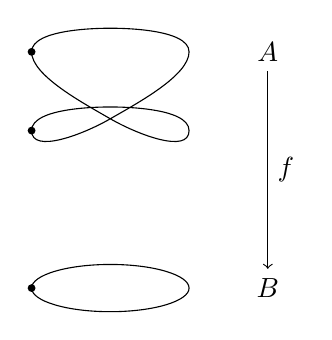
\begin{tikzpicture}
    \node (A) at (2,1) {$A$};
    \node (B) at (2,-2) {$B$};
    \draw[->] (A) -- node[auto] {$f$} (B);
    \draw (0,-2) ellipse (1 and .3);
    \draw (-1,0)
    .. controls ++( 90:-.3) and ++(210: .4) .. (0,0.15)
    .. controls ++(210:-.4) and ++(270: .3) .. (1,1)
    .. controls ++(270:-.3) and ++(  0: .1) .. (0,1.3)
    .. controls ++(  0:-.1) and ++( 90: .3) .. (-1,1)
    .. controls ++( 90:-.3) and ++(150: .4) .. (0,0.15)
    .. controls ++(150:-.4) and ++(270: .3) .. (1,0)
    .. controls ++(270:-.3) and ++(  0: .1) .. (0,0.3)
    .. controls ++(  0:-.1) and ++( 90: .3) .. (-1,0);
    \node[fill,circle,inner sep=1pt] at (-1,-2) {};
    \node[fill,circle,inner sep=1pt] at (-1,0) {};
    \node[fill,circle,inner sep=1pt] at (-1,1) {};
  \end{tikzpicture}
  \caption{A visualization of a covering of the circle}
  \label{fig:covering}
\end{figure}


To sum up with a formula, 
given a type $B$, the type of coverings of $B$ is
$$\sum_{A:\UU}\sum_{f:A\to B}\prod_{b:B}\isset(f^{-1}(b)),$$ 
or equivalently, the type of type families
$$B\to\Set.$$
Note that the identity type  $(A,f,!)=(A',f',!)$ of two coverings is equivalent to 
$$\sum_{p_A:A=_{\UU}A'}(f'p_A=_{A\to B}f).$$
\begin{definition}\label{def:decktrafo}\footnote{postpone}
  Let $f:A\to B$ be a covering.  A symmetry $(A,f,!)=(A,f,!)$ is called a \emph{deck transformation}.
\end{definition}
%specified by a pair $(p_A,p_f)$ with consisting of a $p_A:A=_{\UU}A'$, a $p_f:f'p_A=_{A\to B}f$.

\begin{definition}
  \label{def:universalcover}
  Let $(B,b_0)$ be a pointed connected groupoid.  
The \emph{universal covering} of $B$ is the covering of $B$ given by the family of sets 
  $$P:B\to\Set,\quad P(b)\defequi (b_0=_Bb),$$
or alternatively as the first projection from $P_{b_0}B\defequi\sum_{b:B}(b_0=_Bb)$ to $B$. 
\end{definition}
Note that $(b_0=_Bb)$ is a family of \emph{sets} exactly when $B$ is a groupoid.  
This condition is not necessary for the following important lemma:

\begin{lemma}
  \label{lem:thepathspaceiscontractible}
  Let $(B,b_0)$ be a pointed connected type.  Then $P_{b_0}B\defequi\sum_{b:B}(b_0=_Bb)$ is contractible.
\end{lemma}
\begin{proof}
  ((write))
\end{proof}
This somehow deflates the concept ``universal cover'', since we've just shown that the univesal covering coincides with the constant function $\bn 1\to B$ (with value $b_0$), were it not for the manifold practical value of the formulation that we've given.  
In particular, we recognize the set of symmetries $b_0=_Bb_0$ as the preimage of $b_0$, and ultimately this will show that the study of symmetries coincides with the study of the universal covering.

\subsection{The symmetries of the circle}
\label{sec:symcirc}

\begin{lemma}\label{lem:S1groupoid}
  The circle $S^1$ is a groupoid and $\Sloop^-:\zet\to(\base=_{S^1}\base)$ sending $n$ to $\Sloop^n$ is an equivalence.
\end{lemma}
\begin{proof}
  Since the circle is connected, for any $z,w:S^1$ the type $z=_{S^1}w$ is equivalent to $z=_{S^1}\base$, so it is enough to prove the last statement.  
Define two type families 
$$P,R:S^1\to\UU$$ (actually, both families have values in sets).  
The first is the family defined by $P(z)\defequi(z=\base)$ for $z:S^1$ and the second is defined by the induction priciple for the circle by  % $E(\Sloop)(p)=\trans{}_{z,\base,\base}(p)(\Sloop):(z=\base)$
$R(\base)=\zet$ and $R(\Sloop)=\ua(S):(\zet=\zet)$, where $S$ is the successor function.\footnote{must define.  Shall $\ua$ be visible?}%8.1
Transport defines a function $f:\prod_{z:S^1}(P(z)\to R(z))$, with $f(z)(p)\defequi\trp_{R,p}0$.
((finish!!! e.g. as in the book))
\end{proof}
\begin{remark}
  Through \cref{lem:freeloopspace} we can get a different perspective on the circle which highlights it as a type classifying very simple symmetries.
By \cref{lem:freeloopspace} (moving up one universe), a type family $S^1\to\UU$ is uniquely given by a type $X:\UU$ together with a $p:X=_\UU X$, with no further requirements on $p$.  We have seen one example in \cref{def:zet}, namely the one given by the set $\zet$ of integers together with the element $s:\zet=\zet$ given by the successor.  

The importance of this example will become apparent when we eventually explain that \emph{the circle is equivalent to the component $C$ of $\sum_{X:\UU}(X=_{\UU}X)$ containing $(\zet,s)$}. 

Heading towards this goal, we investigate this component a bit further.  Recall from \cref{sec:identity-types} that, in general, if given elements $x,y,z$ in a type $A$, and two identities $f:x=y$ and $g:y=z$, then transport gives rise to the ``composite identity'' $gf:x=z$ (aka $g\circ f$).    Now, if $(X,f):\sum_{X:\UU}(X=_{\UU}X)$, then an element in the identity type $(\zet,s)=(X,f)$ consists of a $p:\zet=X$ and a proof that the succesor $s:\zet=\zet$  is transported along $p$ to $f:X=X$, that is, an element in $psp^{-1}=_{X=X}f$.  Now, by transport, $psp^{-1}=_{X=X}f$ is equivalent to $fp=_{\zet=X}ps$, and so the identity type $(\zet,s)=(X,f)$ is equivalent to
$$\sum_{p:\zet=X}fp=_{\zet=X}ps.$$ % the equation $fp=ps$ comes from the fact that equality in the identity type means that the transport of $s$ along $p$ is equal to $f$, in other words we have an element in $p^{-1}sp=_{X=X}f$ (which we have translated for convenience to an element in $fp=_{\zet=X}ps$).
Since $\zet$ is a set, this identity type is a proposition and so our component $C$ is a connected groupoid.  

In particular, the type of symmetries $(\zet,s)=_C(\zet,s)$ is equivalent to $\sum_{p:\zet=\zet}sp=ps$.  

This discussion tells us that the following definition makes sense:

\begin{definition}\label{def:S1toC}
  Let $C$ be the component of $\sum_{X:\UU}(X=_{\UU}X)$ containing $(\zet,s)$.
  Let $$c:S^1\to C$$ be defined by $c(\base)\defequi (\zet,s)$ and $c(\Sloop):((\zet,s)=_C(\zet,s))$\footnote{atrictly speaking, this $c$ is $\ap c$ -- I have decided not to distinguish between them; ok?} be given by the successor $s:\zet=\zet$ (and $\refl{}:ss=ss$)
\end{definition}

We are going to prove that $c$ is an equivalence.  This is greatly simplified by the fact that we already know that both $S^1$ and $C$ are connected groupoids, since then \cref{lem:eqofconntypes} says that it is enough to show that $c$ induces an equivalence of symmetries.\footnote{of course, the proof of \cref{lem:S1groupoid} \emph{could} attack $c$ directly, but that would compound the technicalities already present there: at present I prefer splitting it up like this.  I am open for letting the proof of \cref{lem:S1groupoid} be postponed till the end of a chapter, so as not to disrupt the flow of ideas}

\begin{lemma}
  \label{lem:IdCisZet}
  Any element in $(\zet,s)=_C(\zet,s)$ is of the form $(s^k,!)$ for some unique $k:\zet$.  In other words,
  the function 
$$\ev_0:((\zet,s)=_C(\zet,s))\to \zet$$ given by $\ev_0(p)=p(0)$ is an equivalence.
\end{lemma}
\begin{proof}
  Given $(p,!):(\zet,s)=_C(\zet,s)$ we must determine $p:\zet=_{\Set}\zet$, which by univalence amounts to giving all the values $p(n)$ for $n:\zet$.  However, since $sp=ps$ we get that $p(n+1)=p(n)+1$ and so induction on $n$ (induction for positive and negative $n$ separately) gives that $p(n)=n+p(0)$.  Hence, $p=s^{p(0)}$ (uniquely since $\zet:\Set$).
\end{proof}


\begin{theorem}\label{thm:S1bysymmetries}
  The function $c:S^1\to C$ is an equivalence.
\end{theorem}
\begin{proof}
  In view of \cref{lem:eqofconntypes} we only need to show that the induced function of symmetries $c:(\base=_{S^1}\base)\to((\zet,s)=_C(\zet,s))$ is an equivalence.\footnote{ ((can we call equivalences between sets bijections?)).}  

The function $\Sloop^-:\zet\to (\base=_{S^1}\base)$ sending $n:\zet$ to $\Sloop^n$ is an equivalence by  \cref{lem:S1groupoid} and the function  $\ev_0:((\zet,s)=_C(\zet,s))\to \zet$ given by $\ev_0(p)=p(0)$ is an equivalence by \cref{lem:IdCisZet}.  Tracing through the composite function $\ev_0c\Sloop^-:\zet\to\zet$ we see that $\ev_0c\Sloop^n=\ev_0s^n=n$, (\ie $\ev_0c\Sloop^-=\id_\zet$) giving that $c$ is an equivalence. 
% The composition with the functions $\Sloop^-:\zet\to (\base=_{S^1}\base)$ sending $n:\zet$ to $\Sloop^n$ and $\ev_0:((\zet,s)=_C(zet,s))\to \zet$ of \cref{lem:IdCisZet} given by $\ev_0(p)=p(0)$ gives us a function $w:\zet\to\zet$ with $w(n)=s^n(0)$.  From \cref{lem:S1groupoid} we know that $\Sloop^-$ is an equivalence, so we only need to show that $w$ is an equivalence
\footnote{I may have used 2-out-of-3 before, we probably need to include it somewhere, though by univalence it hardly seems necessary}% .  If $p:\zet=\zet$ with $!:sp=ps$, we get by induction on $n:\zet$ (induction for positive and negative $n$ separately) that $p(n)=n+p(0)$.  Hence, all the elements in the preimage $w^{-1}(p,!:sp=ps)$ are equal to $(p(0),!)$.  
\end{proof}

% Now, consider the function 
% $$f:\sum_{p:\zet=\zet}(sp=ps)\to\zet,\qquad f(p,!)=p(0).$$  If $a:\zet$, then $f^{-1}(a)$ consists of the $p:\zet=\zet$ with $sp=ps$ and $p(0)=a$ (the last two are propositions), but by induction we see that $p(n)=n+a$ for all $n:\zet$ (separate induction on positive and negative numbers).  In other words, all elements in the set $f^{-1}(a)$ are equal, and so $f$ is an equivalence


%   ((TODO))
% As an illustration of things to come in a simpler setting, we can give the torsor definition of the circle, where Marc makes the simplifying observation that (since the integers is free on one generator) this can be coded in terms of the successor and there is a priori no need to talk about the abstract group.  In short: an (abstract) $\ZZ$-set is uniquely given by a set $X$ with an identity $f: X=_{\Set}X$.  A $\ZZ$-torsor $(X,f)$ is a $\ZZ$-set (merely) equal to $(\zet,S)$ ($S$ is the successor), that, there is a $p:X=\zet$, so that $Sp=_{X=X} pf$.  This is based at (the pricipal $\ZZ$-torsor represented by) $(\zet,S)$ and $(\zet,S)=(\zet,S)$ consists of $f:\zet=\zet$ s.t. $Sf=fS$.  Such an $f$ must be given by addition by the integer $f(0)$.  This gives us an equivalence between $S^1$ and the type of (secret) $\ZZ$-torsors.  This will be trivial if we have shown that a map of connected groupoids is an equivalence if it induces an equivalence on the identity sets.
\end{remark}

\section{Coverings of the circle}
\label{sec:covS1}

\footnote{The below is not fully structured yet, and does contain known nonsense (basepoints, orientations etc need to be straightened out)}
From \cref{lem:eqandcovofconntypes} we know that a function $f:A\to S^1$ from a connected type $A$ is a covering if and only if for given $a_0:f^{-1}(\base)$ the induced function from $a_0=_Aa_0$ to $(f(a_0)=f(a_0))=(\base=_{S^1}\base)$ is injective; or in words, if the symmetries of $a_0$ inject into the symmetries of $\base$ (which by \cref{lem:S1groupoid} may be identified with with the set $\zet$ of integers).

So, a classification of coverings of the circle amounts to answering the question of what ``subsymmetries'' $\base$ posesses.  Using language yet to be introduced, the question would be ``what are the subgroups of the integers?''

\begin{example}
  \label{ex:listofS1covers}
  In the course of our discussion, we will see that -- under an assumption on the setup called ``LPO'' -- the following represent all the connected decidable coverings of the circle.
  \begin{enumerate}
  \item The \emph{universal} connected cover  $$c_\base:\bn 1\to S^1$$ sends the unique element of $\bn 1$ to $\base$ is a covering corresponding to the trivial symmetry of $\base$ (\ie only $\refl\base$).  
  \item If $m:\NN$ is positive, consider the \emph{degree $m$ function} $$-^m:S^1\to S^1$$ given by $-^m(\base)\defequi\base$ and $-^m(\Sloop)\defequi\Sloop^m$.  On the level of identity types and under the equivalence $\Sloop^-:\zet\simeq(\base=_{S^1}\base)$, this covering corresponds to the function $\zet\to\zet$ given by multiplication by $m$.
  \end{enumerate}
\end{example}

\begin{remark}
  \label{rem:RtoS1}
  The first case, namely the manifestation of the contractible type as a covering of the circle is important in many applications.  Classically it corresponds to the trigonometric functions sending the real number $x$ (the real numbers form a contractible space) to the point $(\cos x,\sin x)$ on the unit circle in the plane.  If you're familiar with complex numbers, you may want to say that this covering is the exponential function sending the real number $x$ to the point $e^{2\pi ix}$ on the unit circle in the complex plane.

  \label{rem:finitecoveringsofS1}
  The analogue of our degree $m$ function is the $m$th power of complex numbers restricted to the unit circle.  The following is perhaps more tangible.  Let $m=12$ and picture the circle and mark $12$ evenly spaced points.  This will look like a clock, with marks $1,2,\dots,12$.  You can then make a function from the circle to itself by sending all marks to $12$ and each of the arcs connecting the marks to the entire circle -- (in a continuous manner preserving the orientation).
  ((picture!!))
\end{remark}

We could be more ambitious and ask: what is the \emph{type} of decidable coverings of the circle?  Since the type of coverings is equivalent to $S^1\to \Set$, and the fact that if $F,F':S^1\to\Set$, then $F=_{S^1\to\Set}F$ is the type $\prod_{z:S^1}(F(z)=_{\Set}F'(z))$ (which is a set\footnote{reference}), we see that the type of decidable coverings of the circle is a groupoid.  We will pin this groupoid down by first identifying the components (of which there turns out to be one for each natural number), and then analyzing one component at a time.

 Recall the function $c:S^1\to C$ of \cref{def:S1toC}.  By \cref{thm:S1bysymmetries} we know that $c$ is an equivalence, so classifying coverings of $S^1$ is equivalent to classifying coverings of $C$.  
We simplify the notation slightly, letting $\pt_C\defequi(\zet,s):C$ (the element corresponding by \cref{def:S1toC} to $\base:S^1$), and allowing ourselves to write $s:\pt_C=_C\pt_C$ instead of the more honest $(s,!):\pt_C=_C\pt_C$ (corresponding to $\Sloop:\base=\base$).


\begin{example}
 \label{ex:listofCcovers}
  Returning to \cref{ex:listofS1covers}, it is instructive to rephraze these connected coverings in terms of $C$.
  \begin{enumerate}
  \item  The universal connected cover is still represented by the constant function
    $$c_{(\zet,s)}:\bn 1\to C$$ that sends the unique element of $\bn 1$ to $(\zet,s):C$.
  \item Assume that $m:\NN$ is positive.  If $X$ is a set and $f:X\to X$ we define the \emph{ $m$th root}
$$\sqrt[m]f:\bn m\times X\to\bn m\times X$$ by setting 
$$\sqrt[m]f(i,x)=
\begin{cases}
  (i+1,x)& \text{for $i<m-1$ and}\\(0,f(x))& \text{for $i=m-1$}.\footnote{this indexing uses the incarnation $\bn m=\{0,1,\dots m-1\}$ and not $\{1,\dots,m\}$: if this is a problem we should change $\bn m$ since the indexing chosen is very convenient later.}
\end{cases}$$ 
Only one $m$th of the time does $\sqrt[m]f$ use $f$ on $X$ (the rest of the time it increases the element in $\bn m$).  This is illustrated in \cref{fig:root} with the shift by $f$ being vertical and the movement along $\bn m$ going around a circle.  
\begin{figure}
  \centering
  \begin{tikzpicture}
    \node (A) at (4,1) {\quad$\sqrt[m]f:\bn m\times X\to\bn m\times X$};
    \foreach \y in {0,1,2}
    { \begin{scope}[shift={(0,\y)}]
        \foreach \x in {0,...,4}
        { \node[fill,circle,inner sep=1pt] at (180+72*\x:1 and .3) {}; }
        \foreach \x in {0,...,3}
        { \draw[-stealth] (180+72*\x:1 and .3) arc(180+72*\x:252+72*\x:1 and .3); }
      \end{scope} }
    \foreach \y in {1,2}
    { \begin{scope}[shift={(0,\y)}]
        \draw[-stealth] (108:1 and .3)
        .. controls ++( 5:-.3) and ++(80:.2) .. (-.7,-.4)
        .. controls ++(80:-.2) and ++(90:.2) .. (-1,-1);
      \end{scope} }
    \draw[-stealth] (108:1 and .3)
    .. controls ++( 5:-.3) and ++(80:.2) .. (-.7,-.4);
    \node (dz) at (-.7,-.7) {\footnotesize$\vdots$};
    \begin{scope}[shift={(0,3)}]
      \draw[-stealth] (-.7,-.4)
      .. controls ++(80:-.2) and ++(90:.2) .. (-1,-1);
      \node (da) at (-.7,0) {\footnotesize$\vdots$};
    \end{scope}
    \draw [decorate,decoration={brace,amplitude=10pt}]
    (-1.1,-.8) -- (-1.1,2.8) node [black,midway,xshift=-20pt] {\footnotesize $X$};
    \draw [decorate,decoration={brace,amplitude=10pt}]
    (1,-1) -- (-1,-1) node [black,midway,yshift=-15pt] {\footnotesize $\bn{m}$};
  \end{tikzpicture}
  \caption{The $m$'th root of an endomorphism}
  \label{fig:root}
\end{figure}
Indeed, iterating $\sqrt[m]f$ we get $(\sqrt[m]f)^m(i,x)=(i,f(x))$; hence the term ``$m$th root'' is apt.

If $f$ is an equivalence, then so is $\sqrt[m]f$:
\begin{enumerate}
\item on one hand $(\sqrt[m]f)(j,y)$ is equal to $(0,x)$ if and only if $j=0$ and $f(y)=x$, so  $(\sqrt[m]f)^{-1}(0,x)$ is equivalent to $f^{-1}(x)$ which is contractible if $f$ is an equivalence, and 
\item on the other, if $i:\bn m$ is not $0$, then $(\sqrt[m]f)(j,y)$ is equal to $(i,x)$ if and only $j+1=i$ and and $y=x$, and so  $(\sqrt[m]f)^{-1}(i,x)$ is equivalent to  a singleton.
\end{enumerate}


Using univalence, the $m$th root construction applies not only to equivalences, but equally well to identities $f:X=_{\Set}X$; resulting in a function 
$$-^m:\sum_{X:\Set}(X=X)\to\sum_{X:\Set}(X=X),\quad -^m((X,f))=(\bn m\times X,\sqrt[m]f).$$
We now focus on  $C$, the component of $\sum_{X:\Set}(X=X)$ containing $(\zet,s)$.
Note that the function $p:\bn m\times \zet\to\zet$ given by $p(i,n)=i+mn$ is an equivalence and that 
$$p\sqrt[m]s(i,n)=i+1+mn=sp(i,n).$$  
Consequently $(\bn m\times\zet,\sqrt[m]s):\sum_{X:\Set}X=_\UU X$ is in the component of $(\zet,s)$, \ie $(\bn m\times \zet,\sqrt[m]s):C$. % In consequence, if $(X,f):C$ (\ie, $(X,f):\sum_{X:\Set}X=_\UU X$ is in the component of $(\zet,s)$) then also $(\sqrt[m]X,\sqrt[m]f):C$, giving rise to the 
Ultimately, we have defined the
 \emph{degree $m$ function} $$-^m:C\to C,\qquad -^m((X,f))=(\bn m\times X,\sqrt[m]f).$$
% , where $$\sqrt[m]X=\bn m\times X$$ and $\sqrt[m]f(i,x)=(i+1,x)$ for $i<m-1$ and $\sqrt[m]f(m-1,x)=(1,f(x))$.  We prove that $-^m((X,f))$ is in the component of $(\zet,s)$ (which was a requirement for elements in $C$).
 % Since we know that $(X,f)$ is in the component of $(\zet,s)$ it is enough consider the element $(p,!):(\sqrt[m]{\zet},\sqrt[m]s)=(zet,s)$ explicitly given by univalence through $p((i,n))=i+mn$ ((check that it gives an equivalence)).

If $(p,!):(X,f)=_C(X',f')$, then 
$$(\id\times p,!):(\bn m\times X,\sqrt[m]f)=(\bn m\times X',\sqrt[m]f')$$ 
is given by % $(\id\times p)(i,x)=(i,p(x))$ (and by 
the fact $!:(\id\times p)\sqrt[m]f=_{\bn m\times X=\bn m\times X'}\sqrt[m]{f'}(\id\times p)$\footnote{$(i,x)$ is taken to $(i+1,px)$ if $i<m-1$ and $(m-1,x)$ is taken to either $(0,f'px)$ or $(1,pfx)$ which are equal by assumption}.  In particular, letting $p\defequi s:\zet=\zet$, we get that $(\id\times s)(i,n)=(i,sn)=(\sqrt[m]s)^m(i,n)$.

This will eventually ((forwardref)) be explained in terms of the \emph{deck transformations} of the degree $m$ covering of the circle being given by the powers of $\sqrt[m]s$ in a nonunique fashion: for any $a:\zet$, the $a$th and the $(a+m)$th power of $\sqrt[m]s$ give rise to the same deck transformation.



 Note that the equivalence $c:S^1\to C$.\footnote{comeback 190104: demonstrate that the descriptions of the coverings of the circle are the same}
  \end{enumerate}
\end{example}
\begin{xca}
  Check the implicit claims in \cref{ex:listofCcovers}.  ((perhaps best to make them explicit?))
\end{xca}
There are many instance of the $m$-th root construction which is of independent interest.  We record the following for future reference.
\begin{definition}
  \label{def:Zetmodm}
  Let $m$ be a positive integer.
  The element $\zet/m:\sum_{X:\Set}(X=X)$ has first projection $\bn m\times\bn 1$ and second projection $\sqrt[m]{\id}$.
\end{definition}
This realizes the cycle $0\mapsto1\mapsto\dots\mapsto m-1\mapsto 0$ in $\bn m$, and so models ``modular arithmetic''.


Any (other) textbook will tell you that these are all the connected coverings of the circle (precisely one for each natural number), but the procedure is unfortunately not constructive: we need a further assumption which is not generally present in our setup, namely

\begin{quote}
  {\bf The Limited Principle of Omniscience} (LPO)\index{LPO}\label{LPO}\footnote{make an environment that principles can fit in and be numbered}If given a function $P:\NN\to\bn 2$, then either $P$ is constant (we have that $\prod_{n:\NN}(P(0)=P(n))$) or there is an $n_0:\NN$ such that $P(n_0)\neq P(0)$.
\end{quote}
LPO is weaker than the law of excluded middle and we are free to assume it as an axiom -- or not.  We will be explicit about where we will use it.


Fix for the moment a connected type $A$ and a decidable covering 
$$f:A\to C$$ (c.f \cref{def:covering}) and an element $\pt_A:f^{-1}(\pt_C)$.  %Assume $(\pt_A,!):f^{-1}(\pt_C)$
%Recall the element 
%$$\pt_C\defequi(s,\refl{ss}):(\zet,s)=_C(\zet,s),$$ which by \cref{def:S1toC} corresponds to $\Sloop:\base=\base$.
By \cref{lem:eqandcovofconntypes}, the fact that $f$ is a decidable covering exactly says that the induced function of identity types
$$g\defequi\ev_0f^=:(\pt_A=_A\pt_A)\to (\pt_C=_C\pt_C)=\zet$$ is injective and decidable.\footnote{say this in a way consistent with the choices of subsets/injections/embeddings}    

Assume LPO.  We are then left with two situations (use that $g$ is injective and decidable): either $\pt_A=_A\pt_A$ is contractible or there is a $p_0:\pt_A=_A\pt_A$ with $g(p_0)$ different from $0$. 

In the former case ($\pt_A=\pt_A$ is contractible), \cref{lem:eqandcovofconntypes} together with the fact that $A$ is connected implies that $A$ itself is contractible.  

On the other hand, if $p_0:\pt_A=\pt_A$ with $g(p_0)$ different from $0$, then either $g(p_0)$ or $g(p_0^{-1})$ is a positive integer.  Hence the set $H^+$ of positive integers in the image of $g$ is nonempty, and so the fact \cref{lem:Nwellordered} that $\NN$ is well ordered implies that $H^+$ has a minimum, \ie there is a $p:\pt_A=\pt_A$ with  $g(p)=m\defequi\min H^+:H^+$.  Furthermore, if $q:\pt_A=\pt_A$ is any element with $0<g(q)$, then  by \cref{cor:arch} there is a $k:\NN$ such that $g(p)k\leq g(q)<g(p)(k+1)$, or equivalently $0\leq g(q)-g(p)k< g(p)$.  Since $g(q)-g(p)k=g(qp^{-k})$ is a nonnegative integer is in the image of $g$ and simultaneously less than the minimum positive value $g(p)$, we must conclude that $g(q)=g(p)k$.

Arguing similarly for the negative values, we reach the conclusion that the image of $g$ in $\zet$ is the subset of multiples of $g(p)=\min H^+$.  Hence, the image of $f^=:(\pt_A=\pt_A)\to(\base=_{S^1}\base)$ is uniquely given by the positive integer $\min H^+$, and is not dependent on $\pt_A$.\footnote{how to say this gently without starting to much fuss regarding commutativity?}  Furthermore, if $p_A:A=_{\UU}A'$, $f':A'\to B$ and $p_f:f'p_A=_{A\to B}f$, then tracing through the argument, we see that the positive number reached through arguing with $f':A'\to B$ remains the same, but there \emph{is} a possibility that $g(p_0)$ changes sign, so that the minimum of $H^+$ is now not attained by $g(p_0)$, but by $g(p_0^{-1})$.\footnote{maybe some HoTT guy can say this less classically.  We also want to say something about the connection to pointed coverings, conjugations etc to clear the path for later applications}

\begin{lemma}
  \label{lem:componentsofcoversofS1}
  Assume the LPO. Given a connected decidable covering of the circle,  there is a unique natural number $m$ so that the connected covering is equal to the connected covering $-^m$ of \cref{ex:listofS1covers}.  This gives an equivalence between $\NN$ and the propositional truncation of the type of connected decidable covering of the circle. 
\end{lemma}


% A natural question is, given $m:\NN$, what does the associated connective covering $f:A\to S^1$ look like?

% We saw that if $m=0$, then the identity types of $A$ were contractible, and so (in view of \cref{lem:eqandcovofconntypes} since $A$ is connected) $A$ is itself contractible.


% If $0<m$, then the injection $g:(\pt_A=\pt_A)\to\zet$ gives an equivalence of $\pt_A=\pt_A$ with the set $m\zet$ of all multiples of $m$.  In particular, if $m=1$, then the injection hits \emph{all} integers, so $g:(\pt_A=\pt_A)\to\zet$ is an equivalence.  Again, by \cref{lem:eqandcovofconntypes} this means that $A\to S^1$ is an equivalence. 
\begin{remark}
  \label{rem:flipthecircle}
  The reader may wonder how the ``orientation reversing'' $c:S^1\to S^1$ given by $c(\base)=\base$ and $c(\Sloop)=\Sloop^{-1}$ fits into the picture.  In our setting it is equal to the identity on $S^1$ (corresponding to $m=1$): Letting also $c:S^1=S^1$ be the identity given by univalence, we have that $\refl{S^1}=c\cdot c$, so that $c$ itself proves that $\id_{S^1}$ and $c$ are equal.
\end{remark}


% More generally, if $0<m$, let $p:\pt_A=\pt_A$ be in the preimage of $m$ under the equivalence induced by $g$  between $\pt_A=\pt_A$ and $m\zet$ (the multiples of $m$).  Define $i:S^1\to A$ by $i(\base)\defequi\pt_A$ and $i(\Sloop)\defequi p$.  Then $i$ is an equivalence since the composite of $\Sloop^-:\zet\to (\base=\base)$, $i^=:(\base=\base)\to (\pt_A=\pt_A)$ and $g:(\pt_A=\pt_A)\to m\zet$ is the equivalence sending $k:\zet$ to $mk:\zet$. 

% The composite $fi:S^1\to S^1$ is then the decidable covering given by $fi(\base)=\base$ and $fi(\Sloop)=\Sloop^m$.   


% Summing up, the type of connected decidable covers of the circle has one component for every $m:\NN$.  The component corresponding to $m=0$ contains the first projection $\sum_{z:S^1}(\base= z)\to S^1$ from the contractible type.  If $0<m$, the component corresponding to $m$ contains the degree $m$ function $-^m:S^1\to S^1$.
\footnote{Some comments have been commented away}

\section{Deck transformations of the circle are ``cyclic'' }
\label{sec:deckS1}

In this section we prove the following result.  The term ``cyclic'' in the chapter heading refers to the fact that we show that the deck transformations are determined by iterations of a single symmetry.  
\begin{theorem}
  \label{thm:coveringsofS1}
  \begin{enumerate}
  \item The type of decidable coverings of the circle by connected types is a groupoid.
  \item Assuming, the LPO the type of decidable coverings of the circle by connected types is the sum of the component containing the universal covering and for each positive integer $m$, the component containing the $m$-fold covering.
  \item The set $c_\base=c_\base$ of symmetries of the universal covering of the circle is equivalent to $\zet$.  

Furthermore, $s:\zet=\zet$ determines a symmetry $$Q^1:c_\base=c_\base$$ so that, considered as an element in $\sum_{X:\Set}X=X$ the pair $(c_\base=c_\base,Q^1)$ is equal to $(\zet,s)$
  \item For positive $m$, the set $-^m=-^m$ of symmetries of the $m$-fold covering of the circle is equivalent to $\bn m$.  

Furthermore, $s:\zet=\zet$ determines a symmetry $$Q^1:-^m=-^m$$ so that considered as an element in $\sum_{X:\Set}X=X$ the pair $(-^m=-^m,Q^1)$ is equal to $\zet/m$ of \cref{def:Zetmodm}.
  \end{enumerate}
\end{theorem}
\begin{remark}\label{rem:thenonuniquenessofgeneratorsofmodulararithmetic1}
  The symmetries called $Q^1$ in \cref{thm:coveringsofS1} are not uniquely determined by the stated property.  
In the case of the universal covering there are two candidates and for the $m$-fold covering there are as many as there are positive integers less than $m$ that does not divide $m$.  
This behavior will be investigated further when we have the proper machinery to put it to good use.
\end{remark}

  \begin{proof}
    \begin{enumerate}
    \item Ut supra ((reference))
    \item Ut supra ((reference))
    \item  ((spell out $Q^1$))
We are going to investigate the set 
$$D_0\defequi\sum_{g:\bn 1=\bn 1}c_\bullet g=c_\bullet$$ 
of symmetries of the universal covering $c_\bullet$ of the circle.  
Our preferred interpretation of $c_\bullet:\bn 1\to C$ is as the first projection from $P\defequi\sum_{(Y,g):C}(\zet,s)=(Y,g)$ to $C$, and the equivalence $c_{((\zet,s),\refl{})}:\bn 1\to P$ % sends the unique point in $\bn 1$ to $(\zet,s):C$ and $\refl{}:(\zet,s)=(\zet,s)$
. 
More generally, for any type $A$ the function $A\to(\bn 1\to A)$ sending $a:A$ to the function $c_a$ sending the unique element in $\bn 1$ to $a$ is an equivalence, and if $A$ is contractible, then every $c_a$ is an equivalence.

   Consequently, $D_0$ is equivalent to
$$\sum_{((Y,g),p):P}(\zet,s)=_C(Y,g)$$ 
which can be rewritten as
$$\sum_{(Y,g):C}((\zet,s)=_C(Y,g))\times((\zet,s)=_C(Y,g))
$$
For any $a,b:A$ the ``shear'' 
$$\mathrm{shear}:((a=_Ab)\times(a=_Ab))\to((a=_Ab)\times(a=_Aa))$$ 
given by $\mathrm{shear}(p,q)\defequi(p,q^{-1}p)$
is an equivalence and
% The function in 
% $((\zet,s)=_C(Y,g))\times(((\zet,s)=_C(Y,g))\to (((\zet,s)=_C(Y,g)\times(\zet,s)=_C(\zet,s))$ sending $(p,q)$ to $(p,q^{-1}p)$ is an equivalence,
so $D_0$ is equivalent to 
$$\sum_{(Y,g):C}((\zet,s)=_C(Y,g))\times ((\zet,s)=_C(\zet,s)).
$$
Using the equivalence $\ev_0:((\zet,s)=_C(\zet,s))\equiv\zet$ of \cref{lem:IdCisZet}, this
 reduces to 
$$D_0\simeq P\times\zet\simeq\zet.$$
    \item ((this does most of (4).  Needs to be proofread))
    Let $m$ be a positive integer.  
Recall the $m$-fold covering, either in the guise $-^m:S^1\to S^1$ of \cref{ex:listofS1covers} or $-^m:C\to C$ of \cref{ex:listofCcovers}.
We are going to investigate the set
$$D_m\defequi\sum_{g:S^1=S^1}-^mg=_{S^1\to S^1}-^m$$  
%$$D_m\defequi\sum_{g:C=C}-^mg=_{C\to C}-^m$$ 
of symmetries of the $m$-fold covering of the circle% , or equivalently, by univalence, $\sum_{t:C\simeq C}-^mt=_{C\to C}-^m$
.  
By univalence and thanks to the equivalence $c:S^1\to C$ of \cref{thm:S1bysymmetries} $(S^1= S^1)$ is equivalent to $(S^1\simeq C)$.
Since being contractible is a proposition, $S^1\simeq C$ is a subtype of $S^1\to C$,
% Thanks to the equivalence $c:S^1\to C$ of \cref{thm:S1bysymmetries} $(C\to C)$ is equivalent to $(S^1\to C)$,
which by \cref{lem:freeloopspace} is ultimately equivalent to $\sum_{(Y,g,!):C}(Y,g,!)=(Y,g,!)$. 
For the moment we'll investigate the simpler type 
$$F_m\defequi\sum_{t:S^1\to C}-^mt=_{S^1\to C}-^mc$$
and on the way discover that if $(t,Q):F_m$, then $t$ is an equivalence, so that $F_m$ actually {\bf is} equivalent to the type $D_m$ we are interested in.

Given If $t:S^1\to C$ is given by $t(\base)\defequi (Y,g,!)$ (where $!$ asserts that $(Y,g)$ lies in the component of $(\zet,s)$)  and $t(\Sloop)=(p,!,!):(Y,g,!)=_C(Y,g,!)$, (where $p:Y=Y$ and $pg=gp$ (an identity in the set $Y=Y$)), we study the type $-^mt=_{S^1\to C}-^mc$.
Spelling out the details we see that $-^mc$ is defined by 
$$-^mc(\base)=(\bn m\times\zet,\sqrt[m]s,!)$$ and 
$$-^mc(\Sloop)\defequi(\id\times s,!,!):(\bn m\times\zet,\sqrt[m]s,!)=_C(\bn m\times\zet,\sqrt[m]s,!)$$   and $-^mt$ is given by $$-^mt(\base)\oldequiv(\bn m\times Y,\sqrt[m]g,!)$$ and 
$$-^mt(\Sloop)\oldequiv(\id\times p,!,!):(\bn m\times Y,\sqrt[m]g,!)=_C(\bn m\times Y,\sqrt[m]g,!).$$

An element in $Q:-^mc=-^mt$ is then given by a 
$$q:\bn m\times\zet=\bn m\times Y$$ so that $\sqrt[m]g\ q=q\sqrt[m]s$ and $q(\id\times s)=(\id\times p)q$ (both in $\bn m\times\zet=\bn m\times Y$). 
Now, the element $$q^{-1}(\id\times s)q=q^{-1}(\sqrt[m]s)^mq=(q^{-1}\sqrt[m]sq)^m$$ in $\bn m\times Y=\bn m\times Y$ is both equal to $\id\times p$ and equal to $(\sqrt[m]g)^m=\id\times g$, proving that $p=g$. 


Consider another element $(t',Q'):F_m$ (as for $(t,Q)$, we spell out $(t',Q')$ in terms of its accompanying $Y'$, $g'$ and $q'$). 
An identity  $R:(t,Q)=_{F_m}(t',Q')$ consists of a $\rho:t=t'$ and an $s:(-^m\rho)Q=_{-^mc=-^mt'}Q'$ (note that this is a proposition), \ie $R$ is given by an $r:Y=Y'$ with 
$$g'r=_{Y=Y'}rg\text{ and }(\id\times r)q=_{\bn m\times Y=\bn m\times Y'}q'(\id\times r).$$  This shows that every $(t,Q):F_m$ is equal to one with $(Y,g)$ being $(\zet,s)$ and $p$ being $s$, and we \emph{could} reduce to this case, leaving to $q$ the entire burden of proof.  
This also shows another thing: the $t:S^1\to C$ fitting in pairs $(t,Q):F_m$ are all equivalences, so that $F_m$ actually is equivalent to the type $\sum_{g:C=C}-^mg=_{C\to C}-^m$ we are trying to understand.

 On the level of equivalences $\zet\simeq Y$, the equation  $\sqrt[m]g\ q=q\sqrt[m]s$ claims that providing $q$ is the same as providing a point $q(0,0):Y$ through the equation  
$$q(i,n)=q((\sqrt[m]s)^{i+nm}(0,0))=(\sqrt[m]g)^{i+nm}q(0,0).$$  For $(i,k)\in \bn m\times\zet$ define $Q^{(i,k)}$ by setting its first projection to be $q^{(i,k)}=(\sqrt[m]g)^{i+km}q$.  
This exhausts all possible $q(0,0):Y$, so we have accounted for all possible $Q$s.

However, there is some redundancy: since $(\sqrt[m]g)^{i+km}=(\sqrt[m]g)^i(\id\times g^k)$, we have that $g^k:Y=Y$ proves that $Q^{i+km}=Q^{i}$.  ((explain why there is no more redundancy)) 

In hindsight we can give concrete descriptions of all the symmetries: for $i=0,\dots m-1$, let $(Y,g)\defequi (\zet,s)$, $p\defequi s$, and $q(0,0)\defequi i$.
    \end{enumerate}
  \end{proof}

  \begin{remark}
    Regarding the deck transformations of the $m$-fold covering of the circle, recall the picture we tried to evoke in \cref{rem:finitecoveringsofS1}.  How can I move my circle with $m$ evenly spaced marked points  (which we now call $0,1,\dots, m-1$ instead of $1,2,\dots 12$ since it fits better with future applications) without disturbing the projection down to the circle (sending all the marked points to $0$).  I can move the marked points, but a marked point has to be sent to a marked point (otherwise the projection down to the circle would be disturbed).  Let's say that mark $0$ is sent to mark $4$.  However, since we have to preserve the projection down to the circle, the arc from $0$ to $1$ must then be sent to the arc from $4$ to $5$.  Continuing in this fashion, we see that we describe a certain rotation of the circle.  Varying $4$ between $0$ and $m-1$ we see that there are exactly $m$ different symmetries of the $m$-fold covering.  Furthemore they are all rotations of the circle by an angle which is a multiple of $2\pi/m$.
  \end{remark}